\documentclass[oneside,a4paper,12pt]{report}
\usepackage{graphicx}
\usepackage{fancyhdr}
\usepackage{dirtree}
\usepackage{listings,xcolor}
\usepackage{hyperref}
\usepackage{mathtools}
\usepackage{caption}
\usepackage{subcaption}

\newcommand{\foldericon}[0]{{\includegraphics[scale=0.03]{folder_icon_navy_blue.png}}}
\newcommand{\folder}[1]{\foldericon\ {#1}}


%\usepackage{biblatex}
\author{Vaibhav Lokhande}

\definecolor{verbgray}{gray}{0.95}

\lstnewenvironment{code}{%
\lstset{backgroundcolor=\color{verbgray},
  frame=single,
  framerule=0pt,
  basicstyle=\ttfamily,
  columns=fullflexible}
  }{}


\begin{document}
\pagenumbering{roman}
%Main Page Start
	\begin{center}
	
		\begin{huge}
			\textbf{Report}
		\end{huge}

		\ \\
		\ \\
		\begin{large}
			Assignment 1
			\ \\
			\textbf{Binary Entropy Analysis Tool}		
		\end{large}		
		\ \\ 
		\ \\
		\ \\
		\ \\ 
		\ \\
		\ \\
		\begin{large}
		Submitted by
		\end{large}
		\ \\
		\begin{normalsize}
		\textbf{Vaibhav Gajanan Lokhande}
		\end{normalsize}
		\ \\
		2017-18
	\end{center}
%Main Page End
\newpage 
\pagestyle{fancy}
\newcommand{\changefont}{%
    \fontsize{8}{10}\selectfont
}
\fancyhf{}
\fancyhead[LE,RO]{\changefont \rightmark} %section
%\fancyhead[RE,LO]{\changefont  \leftmark} %chapter
\fancyfoot[C]{\changefont \thepage} %footer

%Table of Contents Start
\addcontentsline{toc}{section}{Table of Contents}
\tableofcontents
%Table of Contents End
\pagenumbering{arabic}
\newpage
\chapter{Assignment}
\begin{enumerate}
\item Generate a file  containing 100 bytes, the values of 0's.
\item Calculate entropy of this file.
\item Generate another binary file having 50 0's and 50 1's, and calculate entropy.
\item Apply RAR or ZIP and create test3.rar or test.zip and calculate its entropy.
\item Apply encryption of test2.bin and calculate its entropy.
\item Calculate entropy of any windows app like notepad.exe or paint.exe.
\item Try to download a malware file and calculate entropy.
\end{enumerate}
\chapter{Theory}
\textbf{Entropy} is the measure of randomness of data in a message or file. By calculating entropy, we can determine the randomness of data or occurrence of different characters and thus determine the complexity of any message or file. For example a simple text file will have less entropy compared to its compressed form.\\
The entropy is given by formula\\

\begin{center}
{\huge \textbf{$H=-\sum p_{i}* log_{2}(p_{i}) $}}
\end{center}
\ \\ where, \textit{$p_{i}$} is the probability of occurance of character \textit{i}.
\ \\ Using entropy, we can identify the encrypted or compressed executable, which can be used to detect the malware.
\chapter{Code}
The program is developed in matlab.
\\ \\
\textbf{Entropy.m}
\begin{code}
fileName=input('Enter name of file:','s');
file=fopen(fileName,'rb');
fileData=fread(file);
fileLength=length(fileData);
h=histogram(fileData,256);
frequency=h.Values;
fclose(file);
probability=frequency./fileLength;
i=probability>0;
entropy=-sum(probability(i).*log2(probability(i)))
\end{code}

\chapter{Observations}
\begin{tabular}{|l| l | l | l |}
\hline
\textbf{Sr.No.} & \textbf{File Name} & \textbf{Description} & \textbf{Entropy} \\ \hline
1 & test1.bin & File with all 0's and size 100 bytes. & 0\\ \hline
2 & test2.bin & File with 50 0's \& 50 1's and size 100 bytes. & 1\\ \hline
3 & test3.zip & test2.bin compressed to zip. & 3.7898\\ \hline
4 & test2.bin.gpg & Encrypted test2.bin & 7.2973\\ \hline
5 & notepad.exe & Windows notepad application. & 6.9442\\ \hline
6 & test5.bin & File with half 0's \& half 1's and size is 1MB. & 1\\ \hline
\end{tabular}

\begin{figure}
\begin{subfigure}{0.5\textwidth}
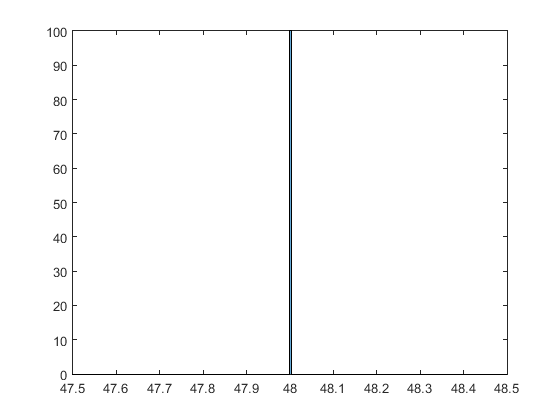
\includegraphics[scale=0.5]{test1.png}
\caption{Result for test1.bin}
\end{subfigure}
\begin{subfigure}{0.5\textwidth}
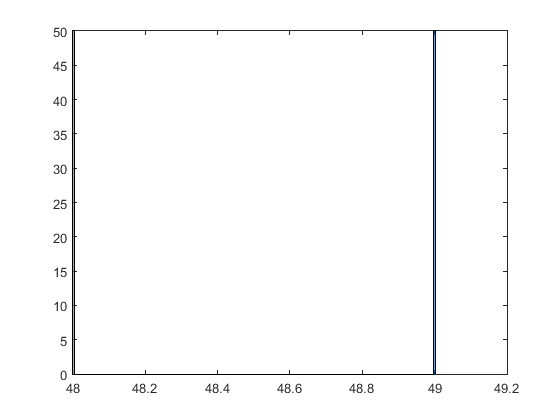
\includegraphics[scale=0.5]{test2.png}
\caption{Result for test2.bin}
\end{subfigure}
\end{figure}

\begin{figure}
\begin{subfigure}{0.5\textwidth}
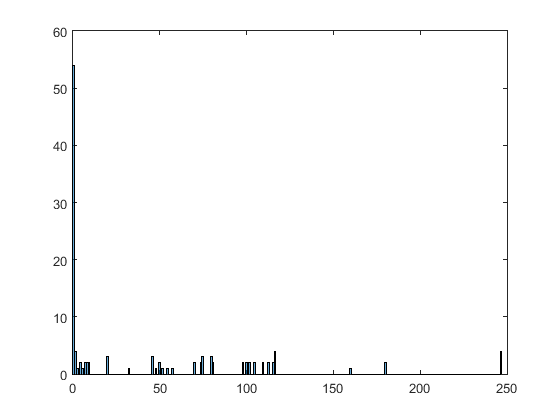
\includegraphics[scale=0.5]{test3.png}
\caption{Result for test3.zip}
\end{subfigure}
\begin{subfigure}{0.5\textwidth}
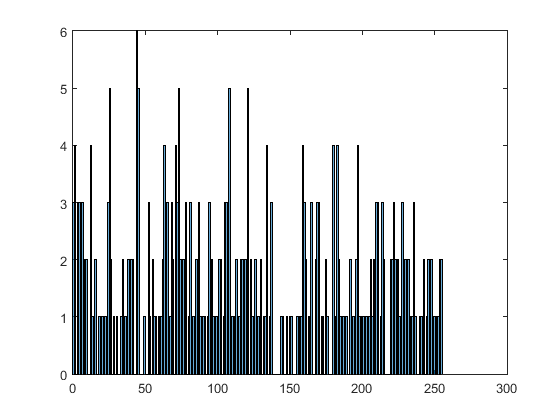
\includegraphics[scale=0.5]{test4.png}
\caption{Result for test2.bin.gpg}
\end{subfigure}
\end{figure}

\begin{figure}
\begin{subfigure}{0.5\textwidth}
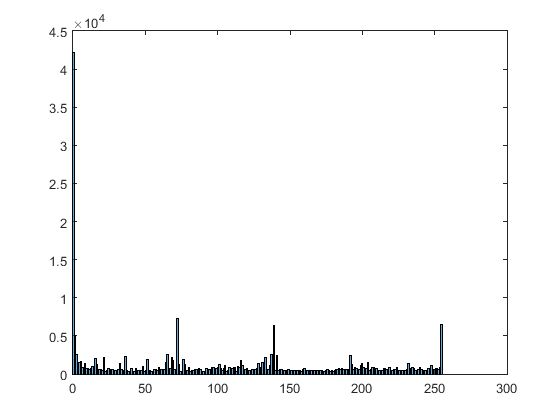
\includegraphics[scale=0.5]{test5.png}
\caption{Result for notepad.exe}
\end{subfigure}
\begin{subfigure}{0.5\textwidth}
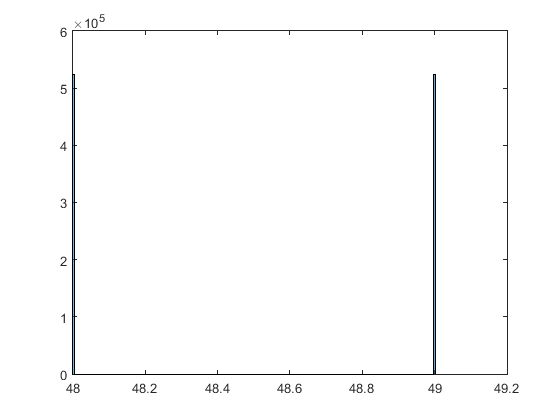
\includegraphics[scale=0.5]{test6.png}
\caption{Result for test5.bin}
\end{subfigure}
\end{figure}


\chapter{Conclusion}
From the observations, we can conclude following points.
\begin{enumerate}
\item Entropy of file increases with increase in randomness of data, 0 when all characters are same and 8 when all characters are different.
\item Entropy file can be anything irrespective of file size. This can be concluded from observation no 2 and 6, where size of file is different but the type of data is same. So their entropy is same.
\item Entropy of encrypted files is very high, more than 7. Using this observation we can determine whether a binary file is encrypted or not.
\end{enumerate}

\end{document}
